%%%%%%%%%%%%%%%%%%%%%%%%%%%%%%%%%%%%%%%%%%%%%%%%%%%%%%%%%%%%%%%%%%%%%
%%                                                                 %%
%% Please do not use \input{...} to include other tex files.       %%
%% Submit your LaTeX manuscript as one .tex document.              %%
%%                                                                 %%
%% All additional figures and files should be attached             %%
%% separately and not embedded in the \TeX\ document itself.       %%
%%                                                                 %%
%%%%%%%%%%%%%%%%%%%%%%%%%%%%%%%%%%%%%%%%%%%%%%%%%%%%%%%%%%%%%%%%%%%%%

%%\documentclass[referee,sn-basic]{sn-jnl}% referee option is meant for double line spacing

%%=======================================================%%
%% to print line numbers in the margin use lineno option %%
%%=======================================================%%

%%\documentclass[lineno,sn-basic]{sn-jnl}% Basic Springer Nature Reference Style/Chemistry Reference Style

%%======================================================%%
%% to compile with pdflatex/xelatex use pdflatex option %%
%%======================================================%%

%%\documentclass[pdflatex,sn-basic]{sn-jnl}% Basic Springer Nature Reference Style/Chemistry Reference Style

%%\documentclass[sn-basic]{sn-jnl}% Basic Springer Nature Reference Style/Chemistry Reference Style
\documentclass[pdflatex,sn-mathphys]{sn-jnl}% Math and Physical Sciences Reference Style
%%\documentclass[sn-aps]{sn-jnl}% American Physical Society (APS) Reference Style
%%\documentclass[sn-vancouver]{sn-jnl}% Vancouver Reference Style
%%\documentclass[sn-apa]{sn-jnl}% APA Reference Style
%%\documentclass[sn-chicago]{sn-jnl}% Chicago-based Humanities Reference Style
%%\documentclass[sn-standardnature]{sn-jnl}% Standard Nature Portfolio Reference Style
%%\documentclass[default]{sn-jnl}% Default
%%\documentclass[default,iicol]{sn-jnl}% Default with double column layout

%%%% Standard Packages
%%<additional latex packages if required can be included here>
%%%%

%%%%%=============================================================================%%%%
%%%%  Remarks: This template is provided to aid authors with the preparation
%%%%  of original research articles intended for submission to journals published 
%%%%  by Springer Nature. The guidance has been prepared in partnership with 
%%%%  production teams to conform to Springer Nature technical requirements. 
%%%%  Editorial and presentation requirements differ among journal portfolios and 
%%%%  research disciplines. You may find sections in this template are irrelevant 
%%%%  to your work and are empowered to omit any such section if allowed by the 
%%%%  journal you intend to submit to. The submission guidelines and policies 
%%%%  of the journal take precedence. A detailed User Manual is available in the 
%%%%  template package for technical guidance.
%%%%%=============================================================================%%%%

\jyear{2022}%

%% as per the requirement new theorem styles can be included as shown below
\theoremstyle{thmstyleone}%
\newtheorem{theorem}{Theorem}%  meant for continuous numbers
%%\newtheorem{theorem}{Theorem}[section]% meant for sectionwise numbers
%% optional argument [theorem] produces theorem numbering sequence instead of independent numbers for Proposition
\newtheorem{proposition}[theorem]{Proposition}% 
%%\newtheorem{proposition}{Proposition}% to get separate numbers for theorem and proposition etc.

\theoremstyle{thmstyletwo}%
\newtheorem{example}{Example}%
\newtheorem{remark}{Remark}%

\theoremstyle{thmstylethree}%
\newtheorem{definition}{Definition}%

\raggedbottom
%%\unnumbered% uncomment this for unnumbered level heads

\begin{document}

\title[Contact Angles of Liquids on Solids]{Lab Report on Contact Angles of Liquids on Solids}

%%=============================================================%%
%% Prefix	-> \pfx{Dr}
%% GivenName	-> \fnm{Joergen W.}
%% Particle	-> \spfx{van der} -> surname prefix
%% FamilyName	-> \sur{Ploeg}
%% Suffix	-> \sfx{IV}
%% NatureName	-> \tanm{Poet Laureate} -> Title after name
%% Degrees	-> \dgr{MSc, PhD}
%% \author*[1,2]{\pfx{Dr} \fnm{Joergen W.} \spfx{van der} \sur{Ploeg} \sfx{IV} \tanm{Poet Laureate} 
%%                 \dgr{MSc, PhD}}\email{iauthor@gmail.com}
%%=============================================================%%

\author*[1,2]{\fnm{Harsh} \sur{Agrawal}}\email{ha1822@ic.ac.uk}

\affil*[1]{\orgdiv{Molecular Bioengineering}, \orgname{Imperial College London}}

%%==================================%%
%% sample for unstructured abstract %%
%%==================================%%

\abstract{The purpose of this experiment was to determine and study contact angles of various different liquids on different solid surfaces, specifically glass slides. These slides were treated with different reagents to modify its surface to analyze differences in contact angles with compared to control. Photographs were taken to measure the contact angles of the different liquids on treated and untreated glass slides; ImageJ software was used for analysis.}

%%================================%%
%% Sample for structured abstract %%
%%================================%%

% \abstract{\textbf{Purpose:} The abstract serves both as a general introduction to the topic and as a brief, non-technical summary of the main results and their implications. The abstract must not include subheadings (unless expressly permitted in the journal's Instructions to Authors), equations or citations. As a guide the abstract should not exceed 200 words. Most journals do not set a hard limit however authors are advised to check the author instructions for the journal they are submitting to.
% 
% \textbf{Methods:} The abstract serves both as a general introduction to the topic and as a brief, non-technical summary of the main results and their implications. The abstract must not include subheadings (unless expressly permitted in the journal's Instructions to Authors), equations or citations. As a guide the abstract should not exceed 200 words. Most journals do not set a hard limit however authors are advised to check the author instructions for the journal they are submitting to.
% 
% \textbf{Results:} The abstract serves both as a general introduction to the topic and as a brief, non-technical summary of the main results and their implications. The abstract must not include subheadings (unless expressly permitted in the journal's Instructions to Authors), equations or citations. As a guide the abstract should not exceed 200 words. Most journals do not set a hard limit however authors are advised to check the author instructions for the journal they are submitting to.
% 
% \textbf{Conclusion:} The abstract serves both as a general introduction to the topic and as a brief, non-technical summary of the main results and their implications. The abstract must not include subheadings (unless expressly permitted in the journal's Instructions to Authors), equations or citations. As a guide the abstract should not exceed 200 words. Most journals do not set a hard limit however authors are advised to check the author instructions for the journal they are submitting to.}

% \keywords{keyword1, Keyword2, Keyword3, Keyword4}

%%\pacs[JEL Classification]{D8, H51}

%%\pacs[MSC Classification]{35A01, 65L10, 65L12, 65L20, 65L70}

\maketitle

\section{Experiment 1}\label{sec1}
\subsection{Introduction}\label{subsec2}

The behavior of a liquid when it interacts with a solid surface depends largely on the interactions that occur in the molecular and nano scales. On  a molecular scale, the surface tension of the liquid determines the strength of interactions between these liquids, whereas on the nano scale, it's the roughness of the surface. Glass, which was used as the solid surface, consists of functional groups such as Silanol (SiOH) that allow it to form hydrogen bonds and thus makes its surface hydrophilic. 

For this experiment, the surface of a glass slide was modified with 1mM octadecyl trichlorosilane (in dichloromethane) to make it hydrophic. Both the modified and the unmodified glass slides included a smooth and a rough surface to evaluate the difference in contact angles due to nano-scale interactions.

Three different liquids with different surface tensions were used to measure contact angles respectively on glass slides.

\begin{table}[h]
\begin{center}
\begin{minipage}{174pt}
\caption{Surface Tension of different liquids}\label{tab1}%
\begin{tabular}{@{}llll@{}}
\toprule
Liquid & Surface Tension\\
\midrule
Water    & 73.0 mN m^{-1}  \\
Glycerol    & 63.4 mN m^{-1}  \\
Propanol    & 23.8 mN m^{-1}  \\
\botrule
\end{tabular}
\footnotetext{The surface tension is recorded at 20^\circ C}
\end{minipage}
\end{center}
\end{table}

\subsection{Observations}\label{subsec2}
Serially $20\mu L$ of all three liquids was added to obtain the contact angles.
\begin{table}[h]
\begin{center}
\begin{minipage}{\textwidth}
\caption{The following table captures the average contact angles taken for Water, Glycerol, and Propanol on different (treated / untreated) glass sldies.}\label{tab2}
\begin{tabular*}{\textwidth}{@{\extracolsep{\fill}}lcccccc@{\extracolsep{\fill}}}
\toprule%
& \multicolumn{2}{@{}c@{}}{Untreated Surface} & \multicolumn{2}{@{}c@{}}{Treated Surface} \\\cmidrule{2-3}\cmidrule{4-5}%
Liquid & Smooth\footnotemark[1] & Rough\footnotemark[2] & Smooth & Rough \\
\midrule
Water  & $5.96^\circ\pm0.64^\circ$ & $8.52^\circ\pm0.60^\circ$ & $58.50^\circ\pm1.40^\circ$ & $74.50^\circ\pm1.50^\circ$\\
Glycerol  & $9.05^\circ\pm0.85^\circ$ & $26.35^\circ\pm0.35^\circ$ & $61.85^\circ\pm0.35^\circ$ & $66.00^\circ\pm1.74^\circ$\\
Propanol\footnotemark[3]  & N.A & N.A & N.A & N.A\\
\botrule
\end{tabular*}
\footnotetext{*Note: Contact angles were measured on both sides of the droplet to get mean and reduce parallax error that may have occurred.}
\footnotetext[1]{For smooth surfaces, the drops of all three liquids were placed side by side due to the availability of a wider space.}
\footnotetext[2]{For rough surfaces, due to the limited space, drops were added one by one followed by cleaning the surface with water and gently tapping out excess fluid with tissues.}
\footnotetext[3]{Contact angles couldn't be inferred for Propanol from the taken photographs on a phone camera.}
\end{minipage}
\end{center}
\end{table}

Parallax error have occurred while collecting the data because the stability of axis on the photograph taken on a phone camera can't be relied upon. 

 \subsection{Images}\label{subsec2}
\begin{figure}[h]%
\centering
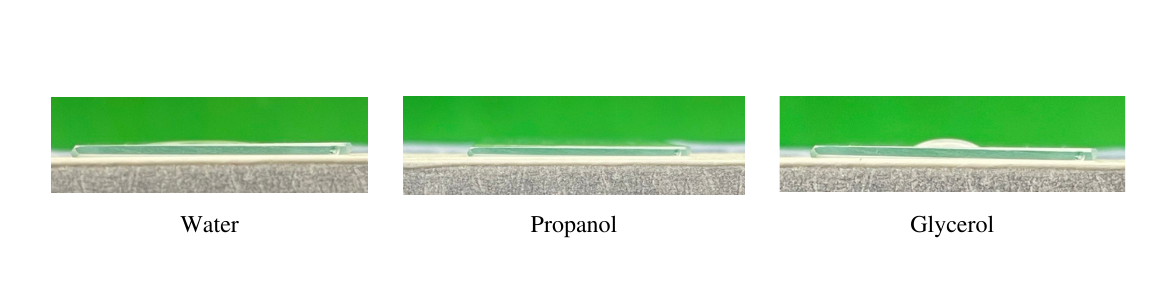
\includegraphics[width=0.9\textwidth]{photos/Untreated_Rough.png}
\caption{Contact angles of Water, Propanol, and Glycerol on the untreated, rough surface.}\label{fig1}
\end{figure}
\begin{figure}[h]%
\centering
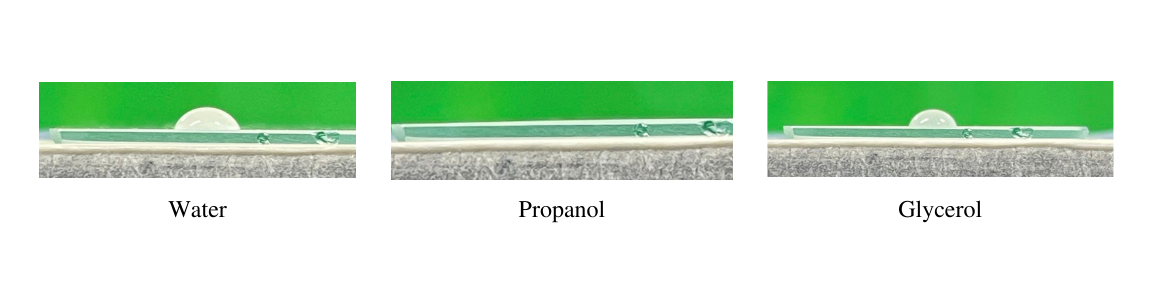
\includegraphics[width=0.9\textwidth]{photos/Treated_Rough.png}
\caption{Contact angles of Water, Propanol, and Glycerol on the treated, rough surface. }\label{fig1}
\end{figure}
\begin{figure}[h]%
\centering
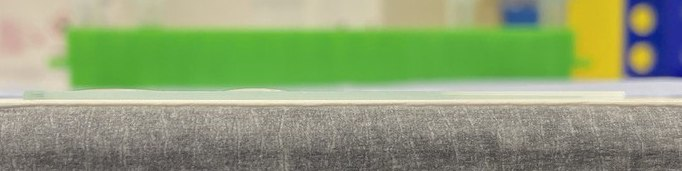
\includegraphics[width=0.9\textwidth]{photos/Untreated_Smooth.jpeg}
\caption{Contact angles of Water, Glycerol, and Propanol on the untreated, smooth surface. }\label{fig1}
\end{figure}
\begin{figure}[h]%
\centering
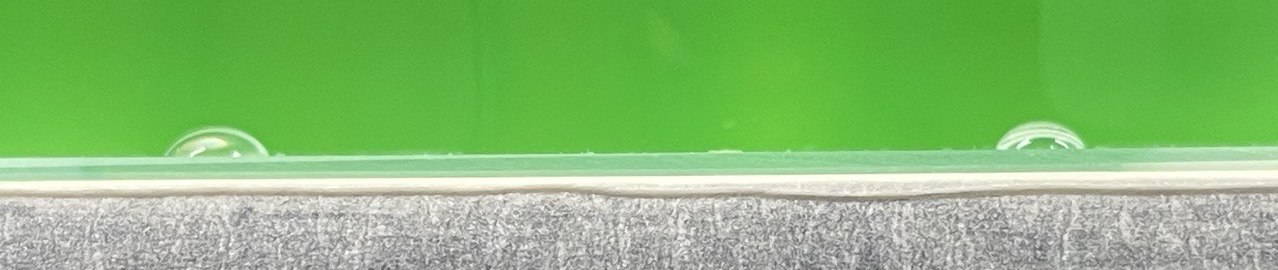
\includegraphics[width=0.9\textwidth]{photos/Treated_Smooth.jpeg}
\caption{Contact angles of Water, Propanol, and Glycerol on the treated, smooth surface. }\label{fig1}
\end{figure}


 \subsection{Inference}\label{subsec2}
\subsubsection{On Untreated Surface}\label{subsubsec2}
Its clearly visible from Figures 1 and 3 that the liquids have a comparatively low angle of contact with the glass slides. Since the glass slide has a hydrophilic surface, it's able to make Hydrogen bonds with the fluids and thus makes it easier for the fluid to wet the surface and flow around easily. 
The contact angle is proportional to the Surface tension and the viscosity of the fluids:
\begin{enumerate}
\item Glycerol has a high surface tension and the highest viscosity amongst the fluids and thus makes a large angle of contact.
\item Water followingly has a higher surface tension than Glycerol but a relatively lower viscosity than it. Thus, it also makes an equally large angle of contact.
\item Propanol on the other hand has a very low viscosity as well as surface tension due to which it makes a negligible angle of contact with the glass slides.
\end{enumerate}

The significant differences in the contact angles between the smooth and rough surfaces of both the treated and untreated surfaces signify the effect of forces acting on the nano-scale. They reinforce the notion that liquids lose mobility in a rougher surface.

\subsubsection{On Treated Surface}\label{subsubsec2}
Upon treatment of the glass slides (silica) with octadecyl trochlorosilane, three SiOH groups of the silica release HCl molecules and conver the surface of the glass slide Hydrophobic. This constricts the formation of Hydrogen bonds between liquids and functional groups present in the surface of the glass slide resulting in an almost 8 - 10x increase in the contact angle.
\begin{enumerate}
\item Unable to form new Hydrogen bonds and having the highest surface tension, water forms the biggest angle of contact. It is roughly 11x greater than the angle of contact of water on the untreated surface.
\item Followed by water, Glycerol also makes a large contact angle with solid surface due to the same phenomena.
\item Unlike the above two, Propanol, still doesn't yield a visible contact angle with the treated silica surface.
\end{enumerate}

The considerable differences in the contact angles between the smooth and rough surfaces of both the treated and untreated surfaces signify the effect of forces acting on the nano-scale. They reinforce the notion that liquids lose mobility in a rougher surface. This effect can greatly be observed with the difference in contact angles made by Glycerol on the smooth, untreated surface ($9.05^\circ\pm0.85^\circ$) vs. rough, untreated surface ($26.35^\circ\pm0.35^\circ$).

\subsection{Sources of Error}\label{subsec2}
\begin{enumerate}
\item A phone camera is unable to provide with stable axis shots of all the images. A tripod with a professional camera with a macro lens is required.
\item While adding drops of liquids on the solid surface, the cleanliness of the surface plays a crucial role. Even though, all precautions to ensure cleanliness were taken, it's impossible to attain ideal conditions.
\item Due to the high viscosity of Glycerol, it's difficult to dispense an exact amount using the micro-pipette tips.
\end{enumerate}

\section{Experiment 2}\label{sec1}
The immobilization of fluorescent labeled BSA protein was carried out in this experiment with glass slides treated with two different functional groups - epoxide and amine. BSA, fluorescent labeled, after immobilization could be viewed under UV light resulting in the visibility of bright yellow spots at the sites of immobilization. 
 
\subsection{Amine Functional Glass Slide}\label{subsec2}
To functionalize with amine, the glass slide was treated with APTES (3-aminopropyltriethoxysilane). Followingly, the glass slide was then immersed in 100mM N, N'-Disucinimidyl Carbonate (DSC) solution. Finally, three drops with increasing volume of BSA were added and the immobilization was viewed under UV. 

\begin{figure}[h]%
\centering
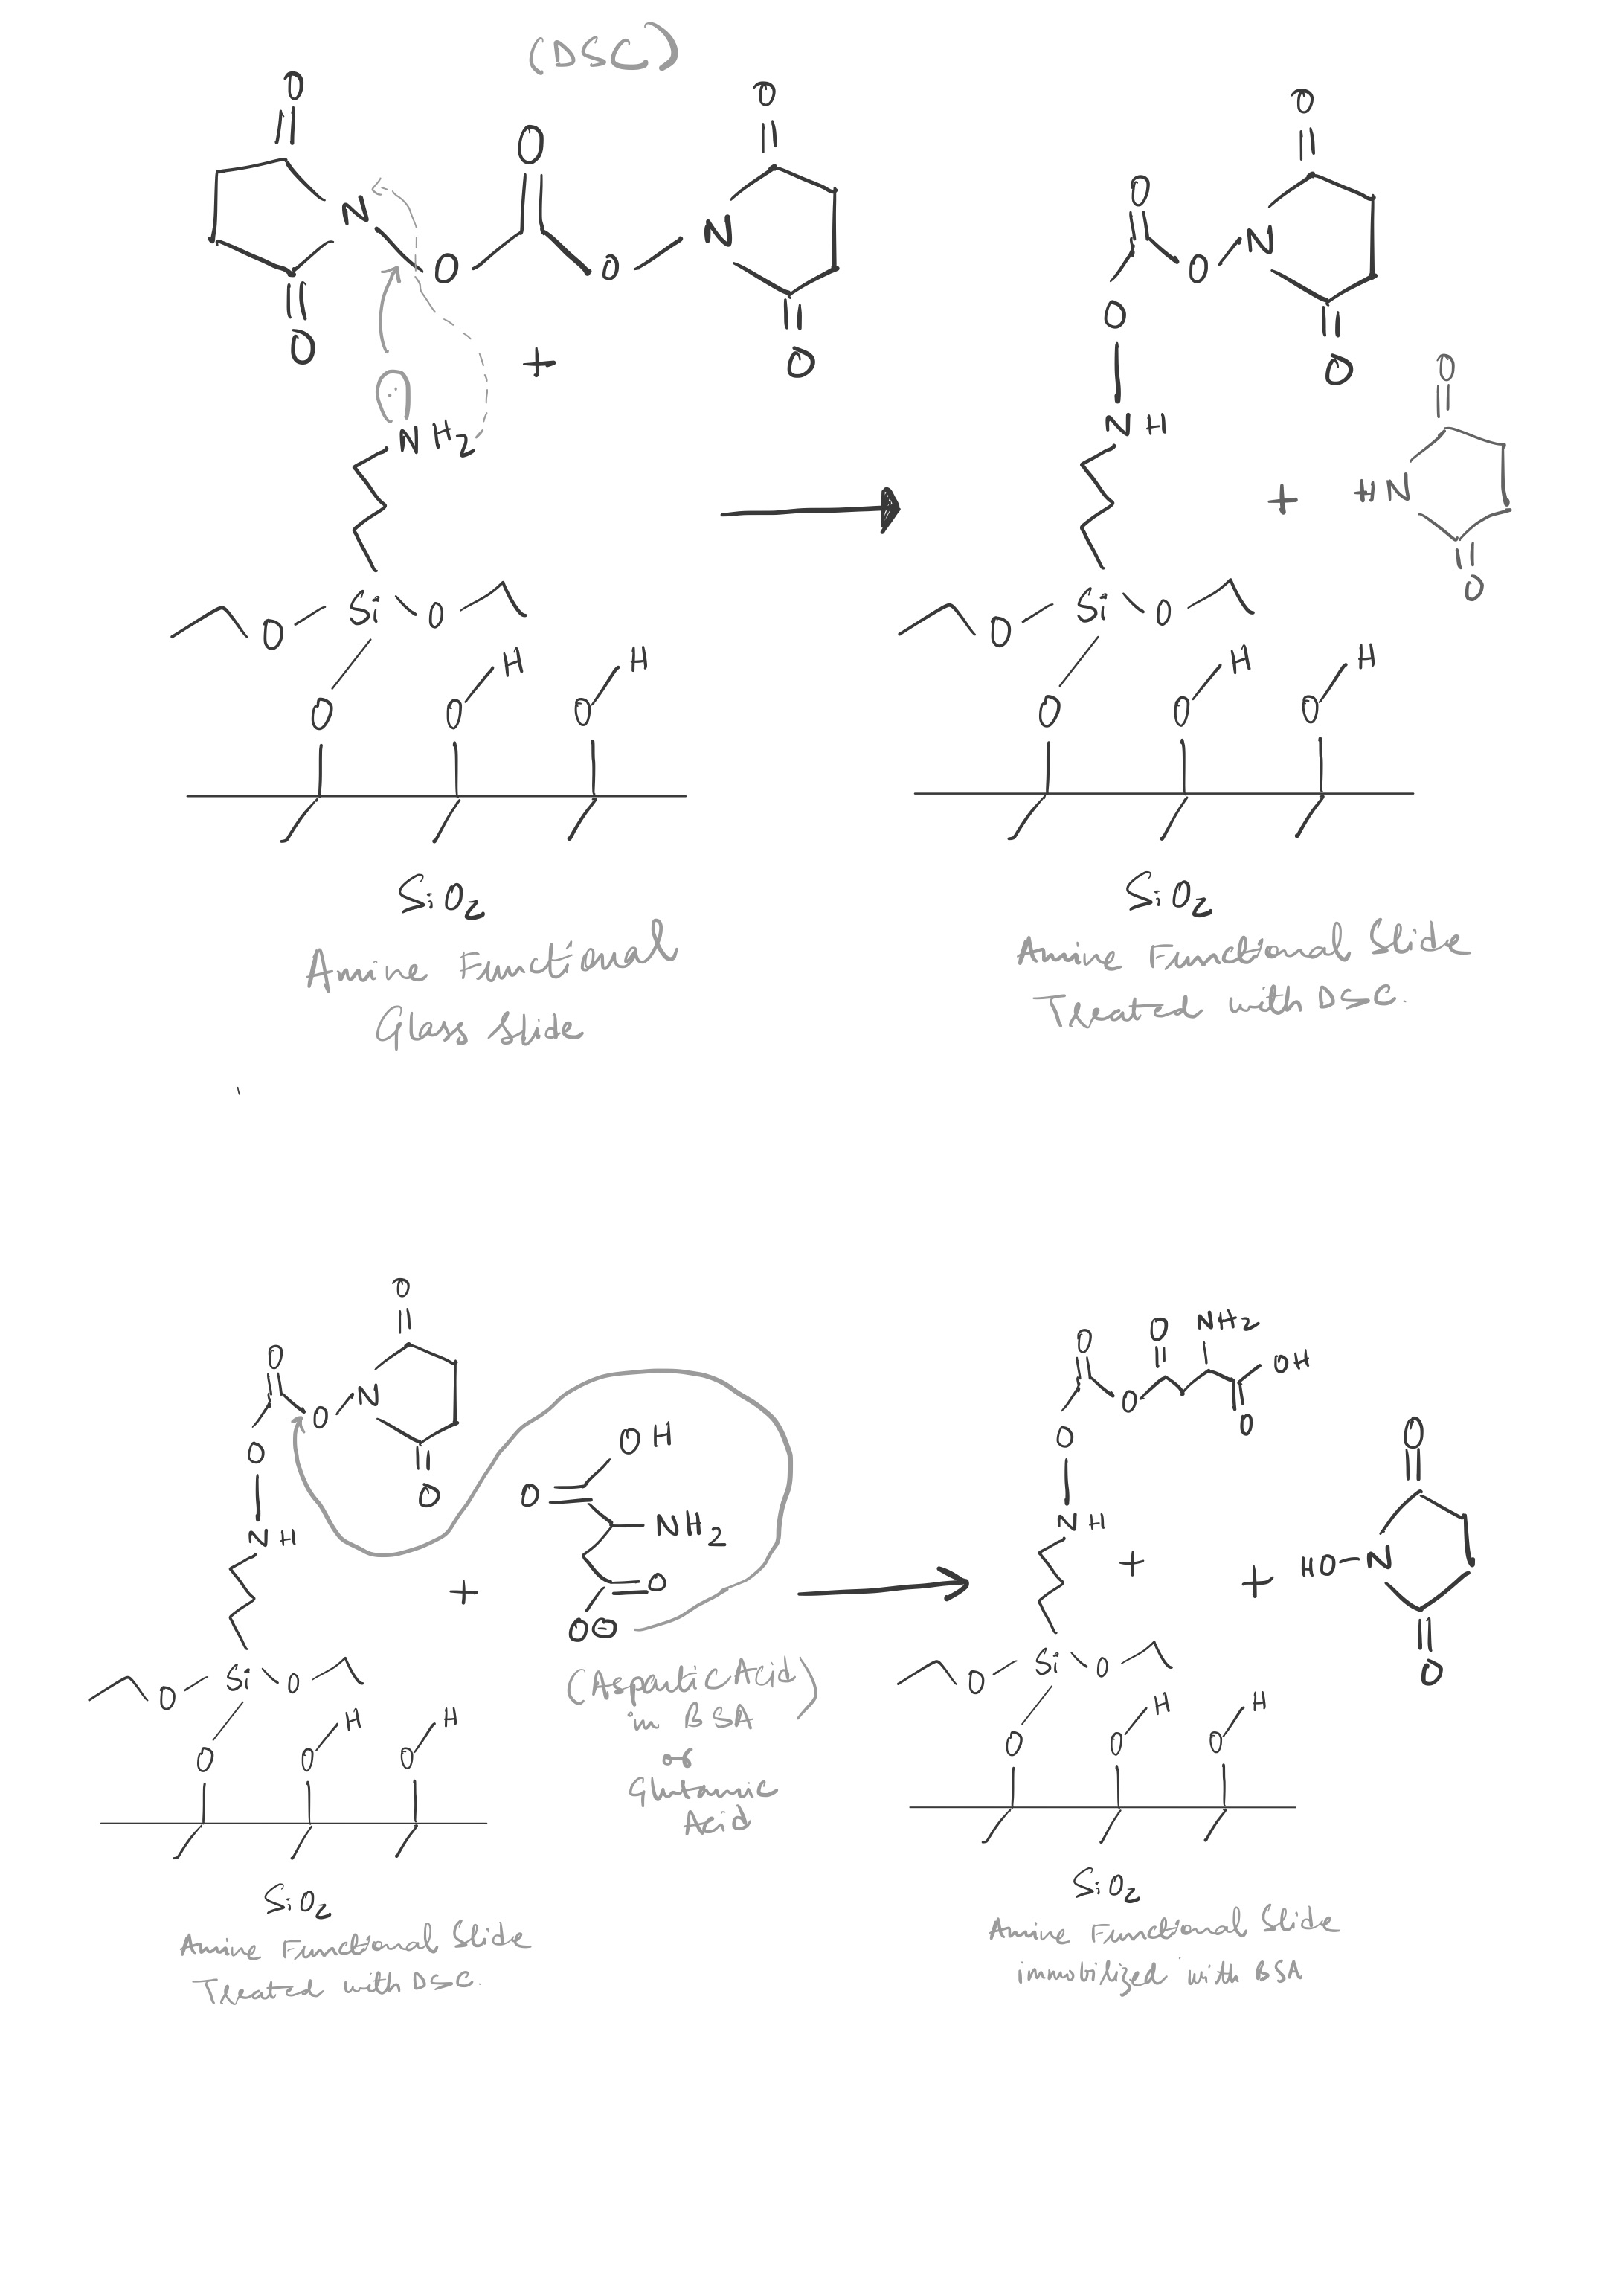
\includegraphics[width=0.9\textwidth]{photos/amine_functional.jpg}
\caption{The following equations show the possible reactions undertaken for BSA immobilization on an amine functional glass slide. }\label{fig1}
\end{figure}
Here, DSC primarily acted as a "ketone" bridge (-O-) to bind the amine functional group of the solid phase to any negative side chain of the BSA protein (Aspartic or Glutamic Acid). Even the uncharged side chains (including Serine and Thrionine), could lose a proton from their hydroxyl group and bind to this ketonic bridge.

\subsection{Epoxide Functional Glass Slide}\label{subsec2}
To functionalize with epoxide, the glass slide was treated with GPTMS ((3-Glycidyloxypropyl)trimethoxysilane). In contrast to the amine functional slide, no intermediary reagent was added. Finally, three drops with increasing volume of BSA were added and the immobilization was viewed under UV. 

\begin{figure}[h]%
\centering
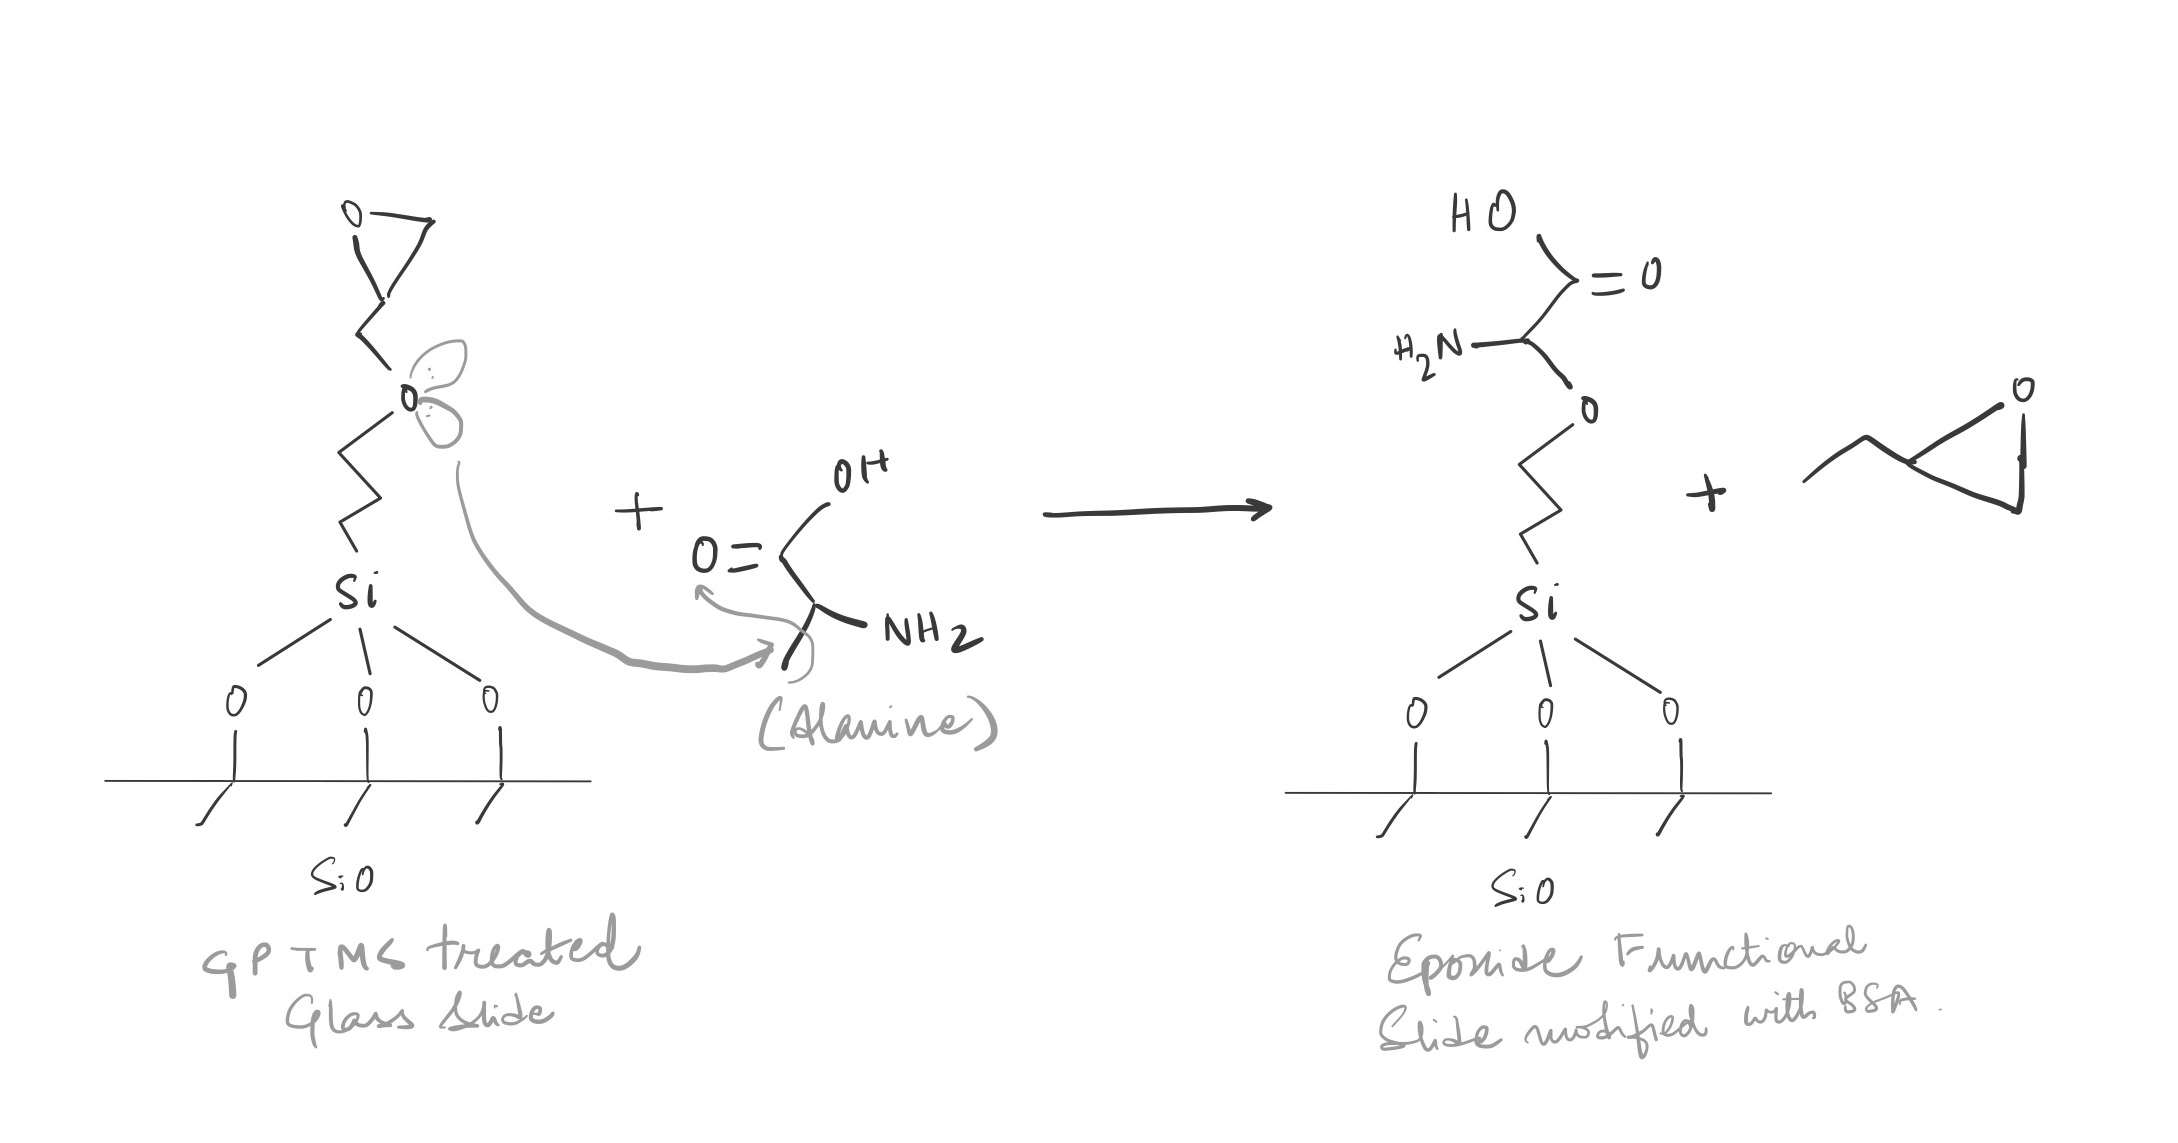
\includegraphics[width=0.9\textwidth]{photos/epoxide.jpg}
\caption{The following equations show the possible reactions undertaken for BSA immobilization on an epoxide functional glass slide. }\label{fig1}

\end{figure}
Under the epoxide functionalized slide, Amino Acids with hydrophobic side chains (Alanine, Valine, Leucine, etc.) present in the BSA protein, lose a proton to bind the Oxygen atom in the GPTMS ketone functional group. This ensures a stable binding of BSA on the epoxide functional glass slide as BSA consists of a significant portion of these amino acids.

\subsection{Sources of Error}\label{subsec2}
\begin{enumerate}
\item One of the most prominent source of error that could prevent the visibility of fluorescent spots of BSA under the UV source could be incorrect conjugation of fluorescent tags with the BSA. Under this condition, even if the immobilization of the BSA occurred, the result wouldn't be visible.
\item Subsequently, the conjugation of fluorescent tags might have occurred on the functional functional groups that were responsible to bind with the glass slides. 
\item Aggressive washing or insufficient incubation time could hinder with the immobilization strength of BSA.
\end{enumerate}

\end{document}
